\documentclass[10pt]{article}

%%%%%%%%%%%%%%%%%%%%%%%%%%%%%%%%%%%%%%%%%%%%%%%%%%%%%%%%%%%%%%%%%%%%%%%%%%%%%%%
%%% packages %%%
%%%%%%%%%%%%%%%%%%%%%%%%%%%%%%%%%%%%%%%%%%%%%%%%%%%%%%%%%%%%%%%%%%%%%%%%%%%%%%%

\usepackage[english]{babel} % Choose english language
\usepackage[labelfont = bf, font = small]{caption} % Use caption package. Use bold font for caption.
\usepackage{siunitx} % Use siunitx for unit representation.
\newcommand{\RM}[1]{\MakeUppercase{\romannumeral #1{:}}}
\usepackage{graphicx}
\usepackage{tabularx}
\usepackage{float}
\usepackage{lmodern}
\usepackage{filecontents}
\usepackage{amsmath}
\usepackage{amssymb}
\usepackage[utf8]{inputenc}
\usepackage[bottom]{footmisc}
\usepackage{leftidx}
\usepackage{subcaption}
\usepackage[explicit]{titlesec}
\usepackage{booktabs}
\usepackage{multirow}
\usepackage{multicol}
\usepackage{listings}
\usepackage{pgfplots}
\usepackage{natbib}
\usepackage{xcolor}
\usepackage{url}
\usepackage{array}
\usepackage{setspace}
\usepackage{hyperref} % Referencing
\usepackage{verbatim}
\usepackage{changepage}
\usepackage[footnote, printonlyused]{acronym}
\usepackage{scrextend}
\usepackage{geometry} % Change geometry of page layout
\usepackage{rotating}
\usepackage{longtable}
\usepackage{lscape}
\usepackage{tocloft}
\usepackage{tkz-euclide}
\usepackage{listings}
\usepackage{feynmp-auto} % Create fenynman diagrams
\usepackage{tikz-feynman} % Create fenynman diagrams
\usepackage{lipsum} % For testing. insert random text

%%%%%%%%%%%%%%%%%%%%%%%%%%%%%%%%%%%%%%%%%%%%%%%%%%%%%%%%%%%%%%%%%%%%%%%%%%%%%%%
%%% new commands and environments %%%
%%%%%%%%%%%%%%%%%%%%%%%%%%%%%%%%%%%%%%%%%%%%%%%%%%%%%%%%%%%%%%%%%%%%%%%%%%%%%%%

% Create custom font
\newenvironment{myfont}{\fontfamily{put}\selectfont}{\par}

% Adapt spacing between lines
\doublespacing

% Delete dots from toc
\renewcommand{\cftdot}{}

% Change section label to roman
\renewcommand{\thesection}{\Roman{section}}

% Customize section layout
\newcommand{\ssection}[1]{%
  \section[#1]{\centering\normalfont\scshape #1}}
\newcommand{\ssubsection}[1]{%
  \subsection[#1]{\centering\normalfont\itshape #1}}
\newcommand{\ssubsubsection}[1]{%
  \subsubsection[#1]{\centering\normalfont #1}}

% Import tikz libraries for figures
\usetikzlibrary{positioning,shadows,arrows}

% Create footnotereferencing
\makeatletter
\newcommand\footnoteref[1]{\protected@xdef\@thefnmark{\ref{#1}}\@footnotemark}
\makeatother

% Change layout of page
\hypersetup{
  colorlinks = true,
  linkbordercolor = {red},
  citebordercolor = {red},
  menubordercolor = {blue},
  urlbordercolor = {blue},
  linktoc = {page},
  pagebackref = {True},
  pdftitle = {Solution 07},
  pdfauthor = {Nils Hoyer, Maurice Morgenthaler},
  pdfcreator  = {pdflatex},
  pdfproducer = {LaTeX}
}

% Change geometry of page
\geometry{a4paper, top = 20mm, left = 20mm, right = 20mm, bottom = 15mm, headsep = 8mm, footskip = 10mm, includeheadfoot}

% Decalre uits for SIunitx
\DeclareSIUnit\femtobarn{fb^{-1}}
\DeclareSIUnit\percent{\%}

% Define colors
\definecolor{deepblue}{rgb}{0,0,0.5}
\definecolor{deepred}{rgb}{0.6,0,0}
\definecolor{deepgreen}{rgb}{0,0.6,0.2}
\definecolor{deeporange}{rgb}{0.9,0.2,0}

%%%%%%%%%%%%%%%%%%%%%%%%%%%%%%%%%%%%%%%%%%%%%%%%%%%%%%%%%%%%%%%%%%%%%%%%%%%%%%%
%%% start document %%%
%%%%%%%%%%%%%%%%%%%%%%%%%%%%%%%%%%%%%%%%%%%%%%%%%%%%%%%%%%%%%%%%%%%%%%%%%%%%%%%

\begin{document}
\begin{myfont}
\lstset{language=C++,
  basicstyle=\ttfamily,
  keywordstyle=\color{blue}\ttfamily,
  stringstyle=\color{red}\ttfamily,
  commentstyle=\color{green}\ttfamily,
  morecomment=[l][\color{magenta}]{\#}
}

\begin{center}
  \begin{Large}
    \textsc{Solution for homework assignment no. 07} \\
  \end{Large}
	\vspace*{0.4cm}
    Nils Hoyer, Maurice Morgenthaler
  \vspace*{1cm}
\end{center}

\section*{Exercise 7.1}

We are asked to determine the expected standard deviation of $\lambda$ where $I(\lambda)$ is the Fisher information and $\hat{\lambda}$ an efficient operator.
The decay time distributions for $\mathcal{B}^{0} \rightarrow J/\Psi K_{s}^{0}$ and $\overline{\mathcal{B}^{0}} \rightarrow J/\Psi K_{s}^{0}$ are
\begin{align*}
N_{\mathcal{B}^{0} \rightarrow J/\Psi K_{s}^{0}} & \propto e^{-t}\left[1 + \lambda\textrm{sin}(\num{0.7}t)\right], \\
N_{\overline{\mathcal{B}^{0}} \rightarrow J/\Psi K_{s}^{0}} & \propto e^{-t}\left[1 + \lambda\textrm{sin}(\num{0.7}t)\right]. \\
\end{align*}

\noindent To calculate the standard deviation we shall use a value of $\lambda =$ \num{0.3}.

\begin{itemize}
  \item[\textbf{a)}] We consider \num{500} decays of $\mathcal{B}^{0}$.

  \item[\textbf{b)}] We consider \num{500} decays of $\overline{\mathcal{B}^{0}}$.

  \item[\textbf{c)}] We consider \num{250} decays of $\mathcal{B}^{0}$ and \num{250} decays of $\overline{\mathcal{B}^{0}}$.

  \item[\textbf{d)}] Put very nice explanation here.
\end{itemize}


\section*{Exercise 7.2}

Given electron tracks we are asked to first plot five tracks into one image.
Afterwards we shall construct a theoretical model for the motion of electrons under the influence of a magnetic field.
Using this model we have to fit it to the given data using a self-written $\chi^{2}$ model.
After plotting different values we eventually state a potential isotope from which the electrons come from. \\

\noindent As usual, please find the script in the text file \texttt{exercise7\_2.C}. \\
You can find the visualisation of the tracks of the first five electrons in figure \ref{fig:ex7_2_tracks}.

\begin{figure}[h]
  \centering
  \caption{Movement of the first five tracks from the file \texttt{exercise07.root}.
  Please not that the \textit{x} and \textit{z} positions are switched to enable fitting.}
  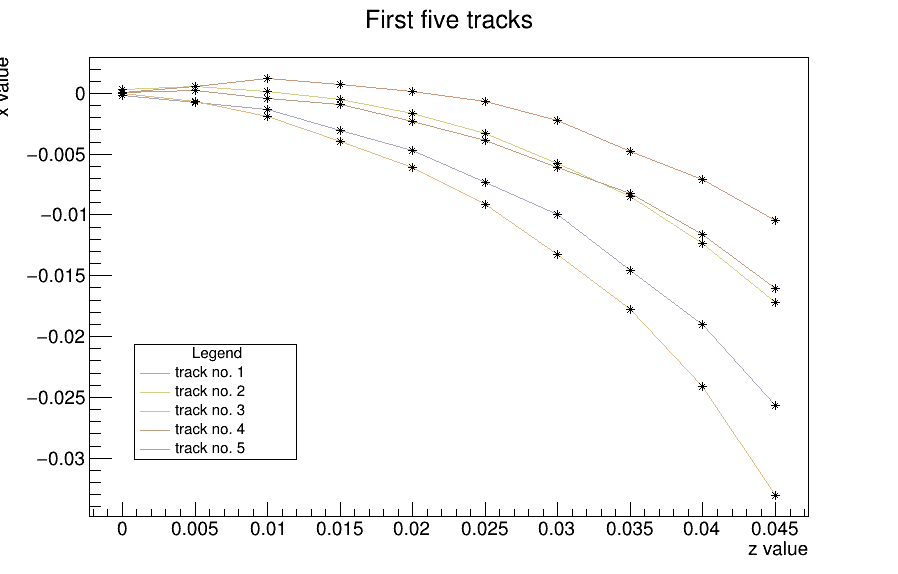
\includegraphics[width = 0.8\textwidth]{./tracks.png}
  \label{fig:ex7_2_tracks}
\end{figure}

\noindent The equation we are looking for have the following expressions

\begin{align}
x  & = - \frac{v_{z} m_{e} \gamma}{c \cdot |q| \cdot |B|} \cdot \textrm{cos}\left(\frac{|q||B|}{m_{e}}\right), \\
y  & = + \frac{v_{z} m_{e} \gamma}{c \cdot |q| \cdot |B|} \cdot \textrm{sin}\left(\frac{|q||B|}{m_{e}}\right),
\end{align}

\noindent where $x^{2} + y^{2} = \left(\frac{v_{z} \cdot m_{e} \cdot \gamma}{c \cdot |q| \cdot |B|}\right)^{2}$ and therefore $y = \sqrt{\left(\frac{v_{z} \cdot m_{e} \cdot \gamma}{c \cdot |q| \cdot |B|}\right)^{2} - x^{2}}$. \\


\end{myfont}
\end{document}
